\documentclass{article}
\usepackage[utf8]{inputenc}

\usepackage{amsmath}
\usepackage{amssymb}
\usepackage{hyperref}%PARA HIPERVÍNCULOS
\usepackage[utf8]{inputenc}
\usepackage[spanish]{babel}
\usepackage[left=3cm,right=3cm,top=3cm,bottom=2.5cm]{geometry}
\usepackage{amsmath,amssymb,latexsym,color,graphicx,verbatim}
\usepackage{afterpage}
\usepackage{mathrsfs}
\usepackage{layout}
\usepackage{graphicx}
\providecommand{\abs}[1]{\lvert#1\rvert} %PARA VALOR ABSOLUTO
\providecommand{\norm}[1]{\lVert#1\rVert} %PARA LA NORMA
\usepackage{mathabx}%PARA LAS FLECHAS DE LOS ESPINES
% $\upuparrows$ -  $\downdownarrows$ - $\updownarrows$ - $\downuparrows$
\usepackage[acronym,shortcuts]{glossaries} %PARA UN GLOSARIO DE ACRÓNIMOS
\makeglossaries
\usepackage[font=small]{caption}
\usepackage[colorlinks = true,  linkcolor = blue,   citecolor = red, urlcolor = blue]{hyperref}

\baselineskip0.75cm
\parskip0.5cm
\parindent0cm


\begin{document}
\begin{titlepage}
\centering {\Large {\sc Resumen Enlace químico y Cristales}}

\vfill
\centering { Resumen realizado para la preparación de la exposición final de la asignatura de Física del Estado Sólido}
\vfill
\hfill

%\centering {\Large Jennifer Grisales Casadiegos \\ Jesús Sánchez Villafrades}

\vfill

\centering {\Large Harol Paredes }




\hfill





\vfill
\vfill

\centering {\Large Universidad Industrial de Santander\\Facultad de
Ciencias\\Escuela de F\'{i}sica\\Bucaramanga\\2020}


\end{titlepage}

\newpage


\begin{abstract}
    ¿Qué mantiene al cristal unido? La interacción electrostática atractiva entre las cargas negativas de los electrones y las cargas positivas del núcleo es completamente responsable de la cohesión entre sólidos. A continuación, veremos un resumen de los fenómenos físicos involucrados en la existencia de los enlaces químicos, la importancia de estos es indiscutible puesto que la vida no existiría sin las interacciones interatómicas e intermoleculares.
\end{abstract}{}



\section{Cristales de gases inertes}
Los gases inertes forman los cristales más simples.  La distribución de electrones es muy cercana de los electrones libres.\cite{Kittel} 

\textbf{Energía de cohesión:} Se define como la energía que debe añadirse a un cristal para separar sus componentes en átomos libres neutros en reposo a una separación infinita.\\

La capa externa de los átomos esta completamente llena y la distribución de electrones es esféricamente simétrica. En el cristal, los átomos de un gas inerte se juntan lo mas cerca posible: fcc, excepto el He3 y He4. La distribución de electrones en el cristal no se distorsiona significativamente de la distribución de electrones  alrededor de átomos libres porque no mucha energía está disponible para distorsionar las distribuciones de energía de átomos libres.

La energía de cohesión de un átomo en el cristal es solo 1\% o menos de la energía de ionización de un electrón en el átomo. Parte de esta distorsión genera la interacción de van der Waals.

En el cristal los átomos de gas inerte se empaquetan tan compactamente como es posible, las estructuras cristalinas son todas cubicas de empaquetamiento compacto (fcc).

Se resumen sus propiedades en el cero absoluto en la siguiente tabla.

\begin{figure}[h]
\centering
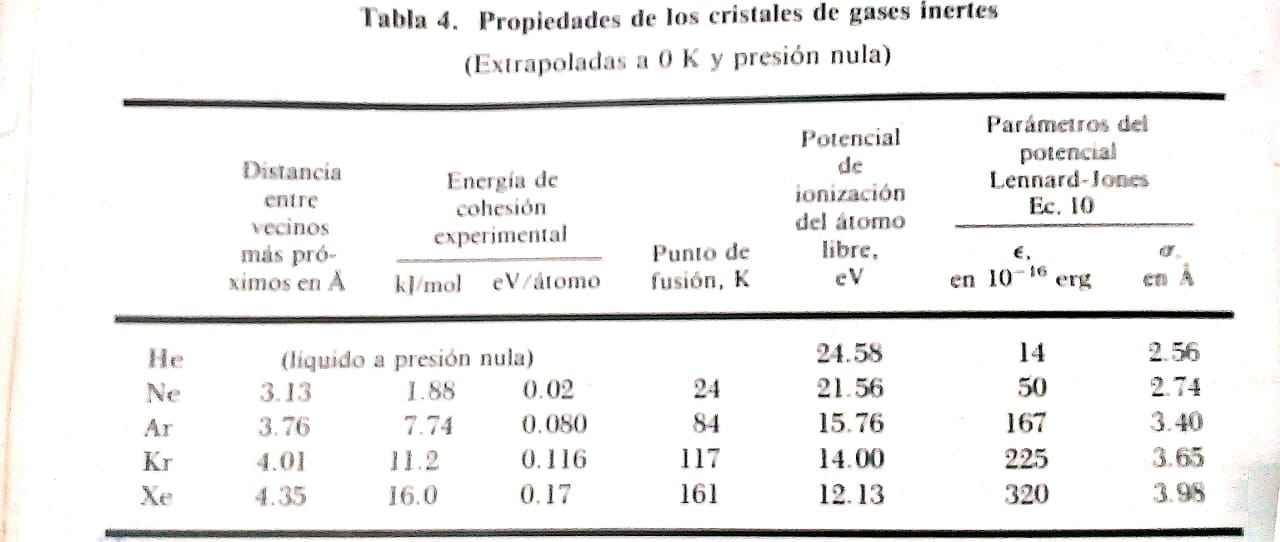
\includegraphics[width=1\textwidth]{a1.jpeg}
\caption{}
\end{figure}

¿Que es lo que mantiene unido un cristal de gas inerte?\\
La distribución electrónica del cristal no puede deformarse de modo significativo respecto a la distribución electrónica que existe alrededor de los átomos libres. Esto se debe a que la energía de cohesión de un átomo del cristal es apenas el 1\% o menos que la energía de ionización de un electrón atómico.

\subsection{Interacción de Van der Waals-London}
Considere dos gases inertes idénticos, con una separación R veces en comparación don el radio de los átomos. ¿Qué interacciones existen entre dos átomos neutros? Si las distribuciones de carga en los átomos es rígida, la interacción entre átomos debería ser cero, porque el potencial electrostático de una distribución esférica de electrones es cancelada fuera del átomo neutro por el potencial electrostático de la carga en el núcleo. Entonces los átomos del gas inerte  podrían no mostrar cohesión y podrían no unirse. Pero los átomos inducen momentos dipolares unos con otros y los momentos inducidos causan una interacción atractiva entre átomos.


Como un modelo, consideremos dos osciladores armónicos lineales e idénticos 1 y 2, separados una distancia R. Cada oscilador soporta cargas $\pm e$ con separaciones $x_{1}$ y $x_{2}$, como en la  figura 1. Las partículas oscilan alrededor del eje x. Sea $p_{1}$ y $p_{2}$ denota el momento. La constante de fuerza es C. Entonces el Hamiltoniano de un sistema sin perturbar eso:


\begin{figure}[h]
    \centering
    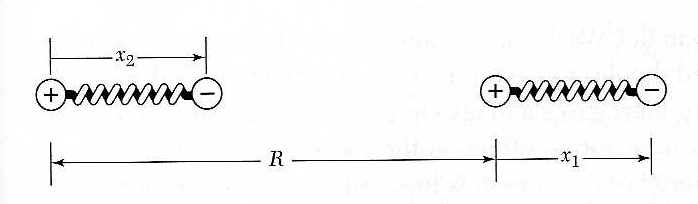
\includegraphics[width=0.8\textwidth]{oscilador.png}
    \caption{Coordenadas de los osciladores}
    \label{Figura 1}
\end{figure}

\begin{equation}
    H_{0} = \frac{1}{2m}p_{1}^{2}+\frac{1}{2}Cx_{1}^{2}+\frac{1}{2m}p_{2}^{2}+\frac{1}{2}Cx_{2}^{2};
        \label{eq1}
\end{equation}{}

Veamos una animación que ilustra mejor esta interacción:
\href{url}{http://virtuallaboratory.colorado.edu/CLUE-Chemistry/LondonDispersionForce/1.2-interactions-0.html}

\begin{figure}[h]
    \centering
    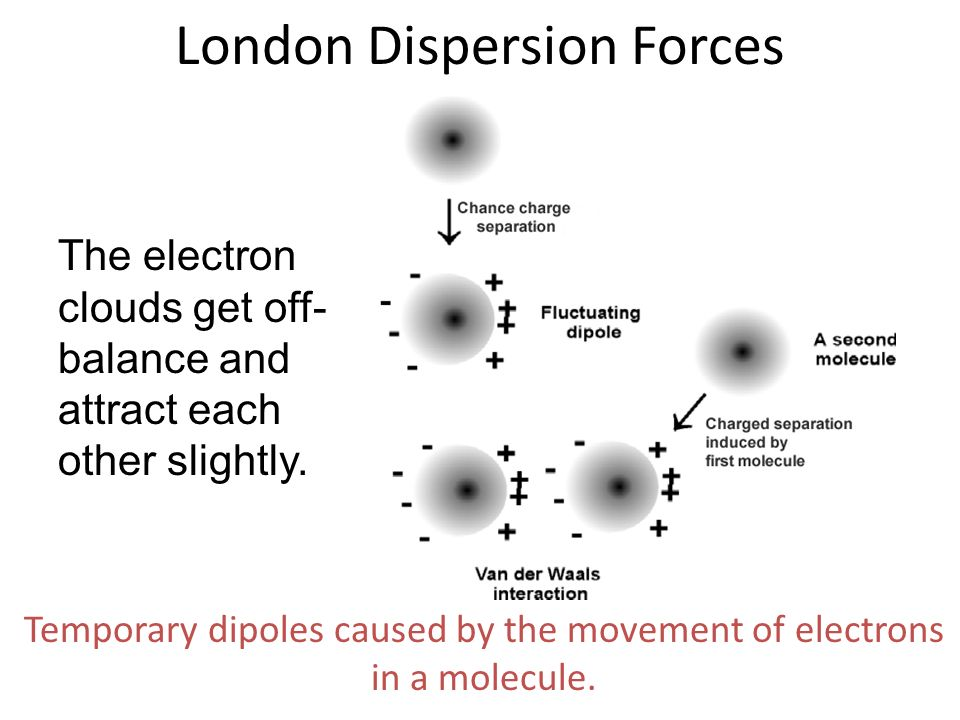
\includegraphics[width=0.5\textwidth]{London+Dispersion+Forces.jpg}
    \label{Figura 1}
\end{figure}

Cada oscilador desacoplado se asume con frecuencia $\omega_{0}$ de la dirección de absorción óptica más fuerte en el átomo. Entonces $C= m\omega_{0}^{2}$.

Sea $H_{1}$ la energía interacción de coulomb de dos osciladores cuya geometría se muestra en la figura. La coordinación intermolecular es R, entonces:

\begin{equation}
    H_{1} =\frac{e^{2}}{R}+\frac{e^{2}}{R+x_{1}-x_{2}}-\frac{e^{2}}{R+x_{1}}-\frac{e^{2}}{R+x_{2}};
    \label{eq2}
\end{equation}

En la aproximación donde $\abs{x_{1}}$, $\abs{x_{2}}$  $R$, expandimos \ref{eq2} para obtener el orden más bajo:

\begin{equation}
    H_{1} \simeq \frac{2e^{2}x_{1}x_{2}}{R^{3}}.
    \label{eq3}
\end{equation}{}

Podemos diagonalizar con la transformación:
\begin{equation}
\begin{split}
&x_{s} \equiv \frac{1}{\sqrt{2}}(x_{1}+x_{2}) , \quad y \\
&x_{a} \equiv \frac{1}{\sqrt{2}}(x_{1}-x_{2}); \\
\end{split}
    \label{eq87687575}
\end{equation}

De igual forma para los momentos diporlares.
\begin{equation}
\begin{split}
    &p_{s} \equiv \frac{1}{\sqrt{2}}(p_{1}+p_{2})\\
    &p_{s} \equiv \frac{1}{\sqrt{2}}(p_{1}+p_{2})
 \end{split}  
\end{equation}{}


Lo cual nos permite tener ahora a $x_{1}$ y $x_{2}$ en términos de modos de movimiento simétrico y antisimétrico y nos permite también obtener el momento. \\
Podemos entonces obtener el Hamiltoniano resultado.\\

\begin{figure}[h]
    \centering
    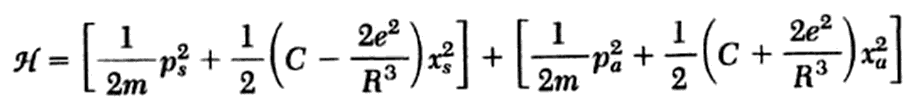
\includegraphics[width=0.7\textwidth]{a4.png}
    \label{Figura 1}
\end{figure}

De esta transformación y consecuentemente las dos frecuencia de los osciladores acoplados serán:

\begin{equation}
    \omega = \left[\frac{C \pm \frac{2e^{2}}{R^{3}}}{m}\right]^{1/2};
        \label{eq4}
\end{equation}\\

Haciendo una expansión binomial:

\begin{equation}
    \omega =\omega_{0}* \left[ 1 \pm \frac{1}{2} \left(\frac{2e^{2}}{CR^{3}}\right) - \frac{1}{8} \left(\frac{2e^{2}}{CR^{3}}\right)^{2} + ... \right];
        \label{eq5}
\end{equation}

El punto cero de energía del sistema es $\frac{1}{2}\hbar (\omega_{s} + \omega_{a})$, porque de la interacción, la suma es reducida de el valor sin acoplar $2*\frac{1}{2}\hbar\omega_{0}$ por:

\begin{equation}
    \Delta U = \frac{1}{2}\hbar (\Delta \omega_{s} +\Delta \omega_{a}) = -\hbar \omega_{0}\frac{1}{8}\left(\frac{2e^{2}}{CR^{3}}\right)^{2} = -\frac{A}{R^{6}}.
        \label{eq6}
\end{equation}

Esta interacción atractiva varía como menos la sexta potencia de la separación de los dos osciladores.

Esta es llamada la interacción de Van der Walls, conocida también como la interacción de London o la interacción inducida dipolo-dipolo. Esta es la principal interacción atractiva en cristales de gases inertes y también en cristales de muchas moléculas orgánicas. La interacción es de efecto cuántico, en el sentido de que $\Delta U -> 0$ como $\hbar -> 0$. De este modo el punto cero de energía es reducido al acople dipolo dipolo dipolo de la ecuación \ref{eq3}. La interacción de van der Waals no depende de la existencia de superposición  de las densidades de carga de los dos átomos.

\subsection{Interacción repulsiva}

Como los dos átomos se mueven juntos, sus distribuciones de carga gradualmente se superponen, de este modo, cambian la energía electrostática del sistema. Con separaciones suficientemente bajas, la energía de solapamiento es repulsiva, en gran parte a causa del principio de exclusión de Pauli. 

\begin{figure}[h]
    \centering
    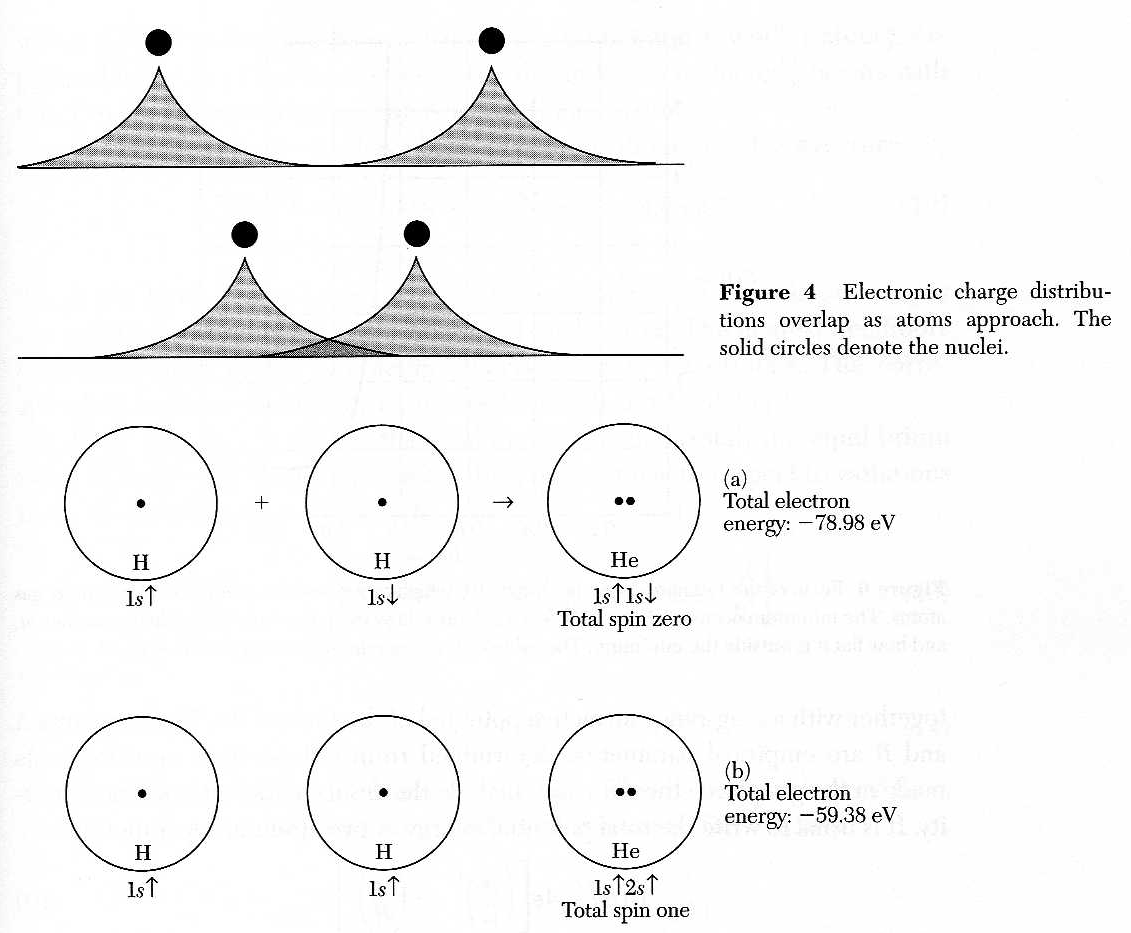
\includegraphics[width=1\textwidth]{superposicion_densidades.png}
    \caption{Efecto del Principio de Pauli sobre la energía de repulsión en un ejemplo extremo, se empujan acercándose dos átomos de hidrógeno hasta que los protones están casi en contacto. En (a), los electrones tienen espines antiparalelos y el principio no actúa. En (b) los espines son paralelos: El principio de Pauli fuerza a que un electrón se promociones desde el orbital 1s del H hasta un 2s del He.}
    \label{Figura 1}
\end{figure}

EL principio de exclusión de Pauli previene de la ocupación múltiple, y la distribución de átomos de capas cercanas pueden superponerse solo si se acompaña con la transición de electrones a desocupados a mayores estados de energía de los átomos. De tal forma el electrón superpuesto incrementa la energía total del sistema y aporta a la contribución repulsiva de la interacción. 


Datos experimentales correspondientes a gases inertes se ajustan muy bien a un potencial repulsivo empírico de la forma: $\frac{B}{R^{12}}$, donde B es una constante positiva.
Si se usa el potencial atractivo  de la ecuación (7) se puede escribir la energía potencial total de dos átomos a una separación R como :\\

\begin{equation}
    U(R)=4\epsilon\left[\left(\frac{\sigma}{R}\right)^{12}-\left(\frac{\sigma}{R}\right)^{6}\right];
\end{equation}{}

Este potencial se conoce como el potencial de Lennard-Jones.Y tiene la forma de la fugura 4. \cite{Maza}

\begin{figure}[h]
\centering
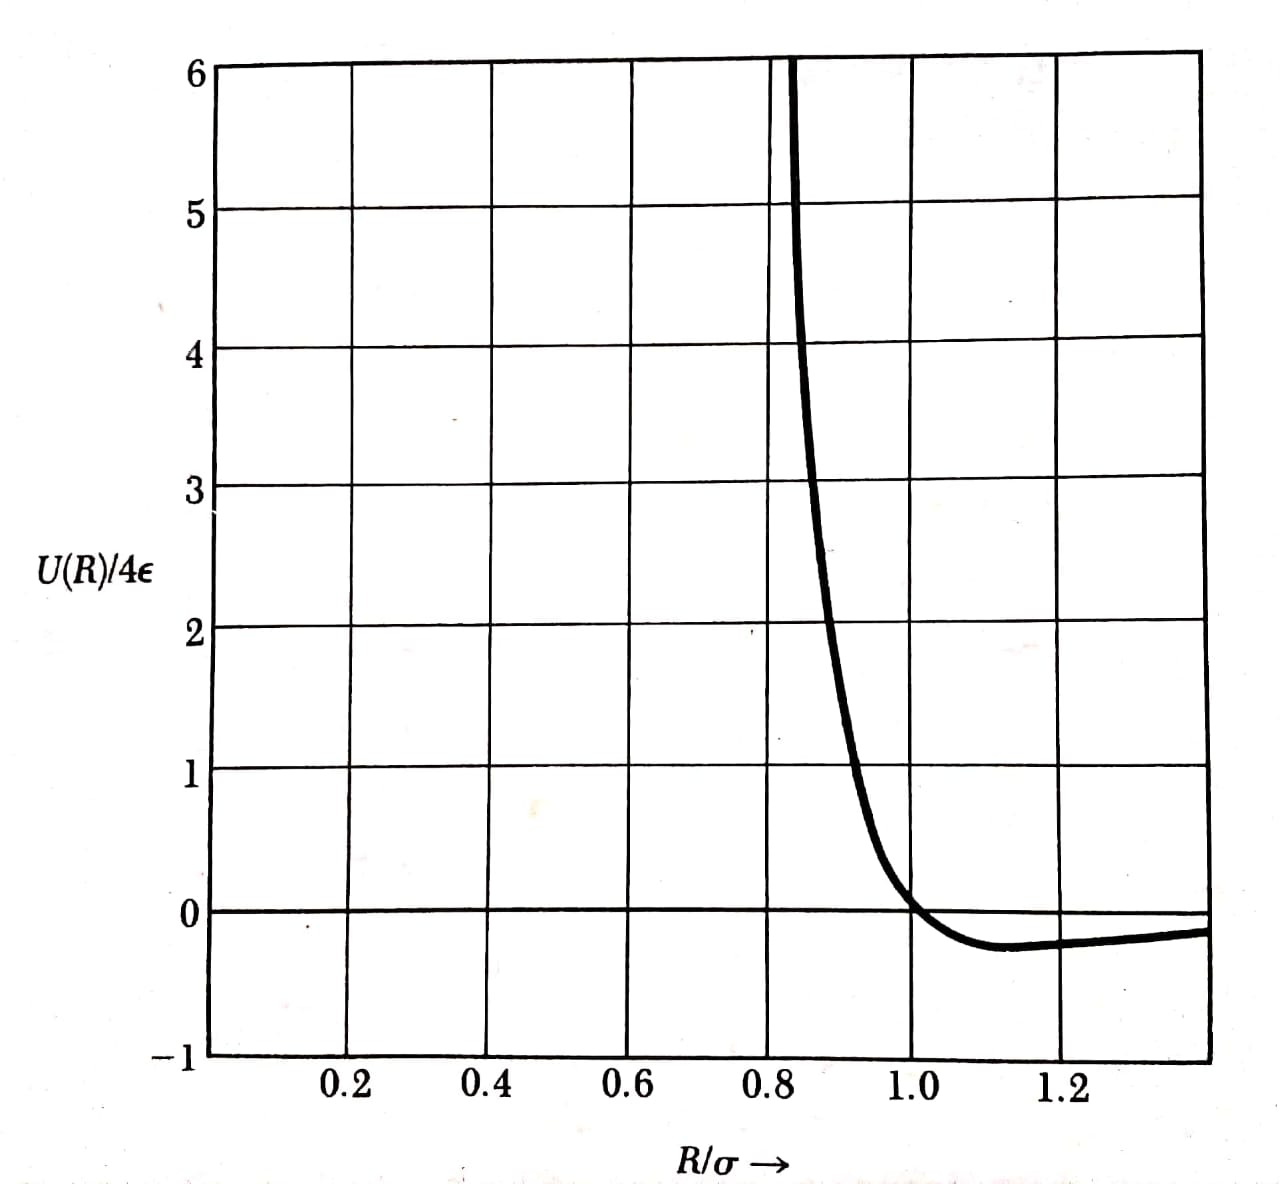
\includegraphics[width=0.8\textwidth]{a2.jpeg}
\caption{}
\end{figure}




\subsection{Constante de equilibrio de la red}

\begin{figure}[h]
\centering
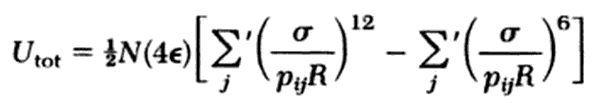
\includegraphics[width=0.4\textwidth]{a3.png}
\end{figure}

La relación $\frac{R_0}{\sigma}$ para los átomos mas ligeros es:
%\begin{figure}[h]
%\centering
%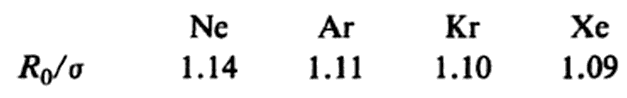
\includegraphics[width=0.4\textwidth]{a5.png}
%\end{figure}
\\
\subsection{Energía de cohesión}

El cálculo de la energía de cohesión es general para los gases inertes dista en un 28, 10,6,4 \% para en Ne, Ar, Kr, Xe respectivamente.Esto es debido a la corrección mecánico-cuantica.\\



\newpage

\section{Cristales Iónicos}

Los cristales iónicos están hechos de iones positivos y negativos. El enlace iónico resulta de la interacción electrostática  de iones de carga opuesta. Dos estructuras cristalinas comunes encontradas para cristales iónicos, el cloruro de sodio  y el cloruro de cesio.

Las configuraciones electrónicas de todos los iones de un cristal iónico simple corresponde a capas electrónicas completas como en el caso de los atomos de gases inertes. Los átomos de gases inertes tienen cortezas completas y la distribución de carga poseen una simetría esférica lo que se espera para cada ion de un cristal iónico , que tenga aproximadamente una simetría esférica, esto se confirma mediante el estudio por rayos x  de la distribución de electrones del NaCl.

\begin{figure}[h]
\centering
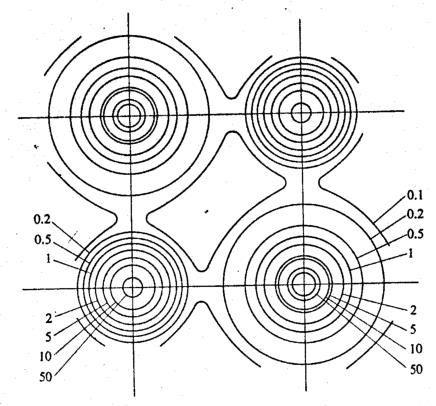
\includegraphics[width=0.5\textwidth]{a6.png}
\caption{}
\end{figure}

Una estimación rápida  nos muestra que si podemos considerar las interacciones electrostáticas formadas en gran parte por la energía de enlace de un cristal iónico.\\

Representación gráfica del enlace iónico del NaCl.

\begin{figure}[h]
\centering
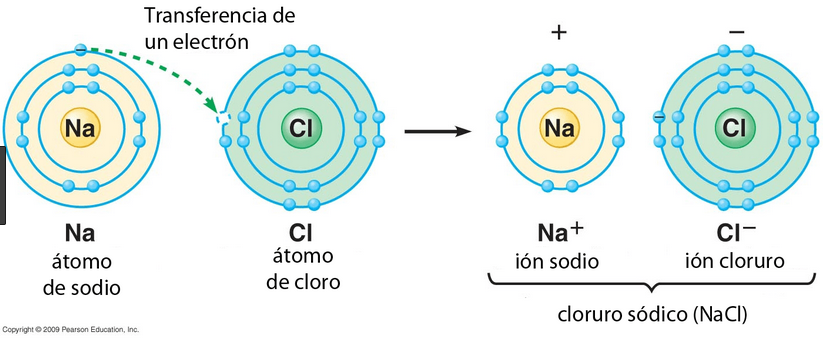
\includegraphics[width=0.8\textwidth]{a11.png}
\caption{}
\end{figure}



\begin{figure}[h]
\centering
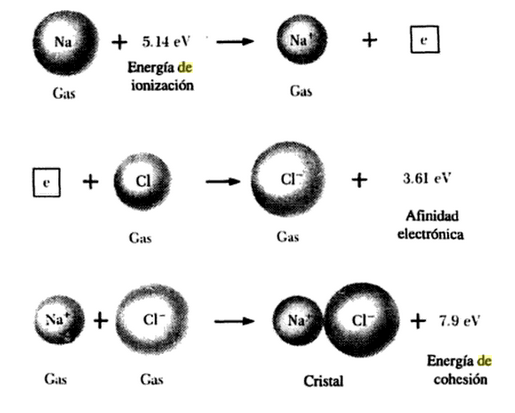
\includegraphics[width=0.6\textwidth]{a7.png}
\caption{}
\end{figure}

\subsection{Energía electrostática o de Madelung}

Las interacciones de largo alcance entre iones de carga $\pm q$ es la interacción electrostática de tipo culumbiano $\pm\frac{q^2}{r}$. Las interacciones repulsivas entre entre estos iones con configuraciones de gases inertes son semejantes a las correspondientes a los mismos átomos de gases inertes. La contribución principal a la energía de enlace en los cristales es electrostática y se denomina \textbf{energía de Madelung}.

Se define $U_{ij}$ como la energía de interacción entre los iones i y j. $U_i$ incluye todas las interacciones en las que interviene el ion i.

\begin{equation}
   U_{i}= \sum_{j} U_{ij} ,
 \label{eq2}
\end{equation}{}

Se supone que $U_{ij}$ puede escribirse de la siguiente forma:

\begin{equation}
   U_{ij}=\lambda e^{(\frac{-r_{ij}}{\rho})}\pm \frac{q^2}{r_{ij}} 
    \label{eq2}
\end{equation}

Se toma el signo (+) para cargas iguales y el (-) para cargas diferentes.\\

Despreciando los efectos superficiales escribimos la energía total de la red de un cristal  compuesto de N moléculas o 2N iones como: $U_{total}=NU_i$ Si se incluye la interacción repulsiva únicamente entre vecinos mas próximos la energía total se escribe como:\\

\begin{equation}
   U_{ij}=NU_i 
    \label{eq2}
\end{equation}

\begin{equation}
   U_{ij}=N\left[z\lambda e^{(\frac{-R}{\rho})}-\alpha\frac{q^2}{r_{ij}} )\right]
    \label{eq2}
\end{equation}

Donde z es el numero de vecinos mas próximos de cualquier ion y 

\begin{equation}
 \alpha = \sum_{j}^{} '\frac{(\pm)}{p_{ij}} \equiv Madelung
\label{eq2}
\end{equation}

Se define como la constante de Madelung.

A continuación se relacionan algunos de los valores típicos de la constante de Madelung.\\\\\\\\

\begin{figure}[h]
\centering
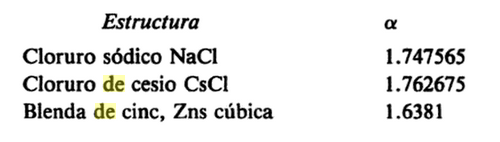
\includegraphics[width=0.6\textwidth]{a9.png}
\caption{}
\end{figure}

La contribución de Madelung y Repulsiva en los enlaces de un cristal de KCl se indican en la siguiente Gráfica.

\begin{figure}[h]
\centering
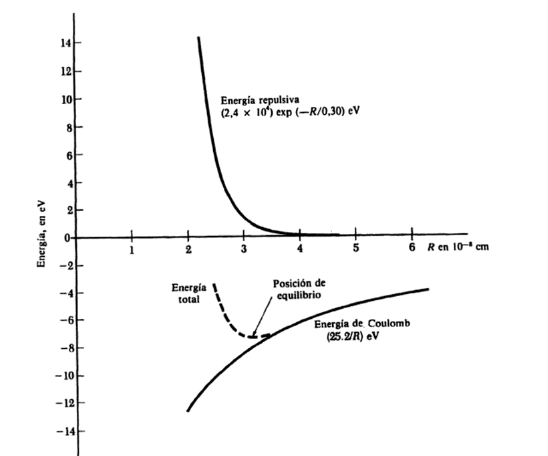
\includegraphics[width=0.6\textwidth]{a10.png}
\caption{}
\end{figure}


\section{Cristales Covalentes}

El enlace covalente entre dos átomos es muy común en los compuestos orgánicos, involucra a electrones de valencia que son compartidos. Este solapamiento asociado de carga electrónica en la dirección de unión de los átomos genera un enlace fuerte. 

El enlace covalente normalmente está formado por dos electrones, uno de cada átomo que participa en el enlace. Los electrones que forman el enlace tienden a estar parcialmente localizados en la región situada entre los dos átomos unidos por dicho enlace. \cite{Hofmann}

Para comprender mejor esto, debemos comprender los fundamentos de la teoría de orbitales moleculares:

\subsection{Teoría de Orbitales Moleculares}

la teoría de los orbitales moleculares (TOM), es un método para determinar el enlace químico en el que los electrones no están asignados a enlaces individuales entre átomos, sino que se mueven bajo la influencia de los núcleos de toda la molécula.

En esta teoría, cada molécula tiene un grupo de orbitales moleculares, y se asume que la función de onda $\Phi f$ del orbital molecular está escrita de manera aproximada como una simple combinación lineal de los n orbitales atómicos constituyentes $\chi_{i}$, de acuerdo con la siguiente ecuación:

\begin{equation}
    \Phi_{j} = \sum_{i=1}^{n} c_{ij}\chi_{i},
\end{equation}

Los coeficientes $c_{ij}$ pueden ser determinados numéricamente por sustitución de esta ecuación en la de Schrödinger y la aplicación del principio variacional. Este método se llama \textbf{combinación lineal de orbitales atómicos} y se utiliza en la química computacional. 

De acuerdo con la teoría de los orbitales moleculares, los enlaces covalentes de las moléculas se forman por solapamiento de orbitales atómicos, de manera que los nuevos orbitales moleculares pertenecen a la molécula entera y no a un solo átomo. 

Recodemos que la forma de los orbitales atómicos está determinada por el número cuántico azimutal $l$ o momento angular orbital.

Por ejemplo para el Nitrógeno: \href{url}{https://i.gifer.com/IYAr.gif}

\begin{figure}[h]
\centering
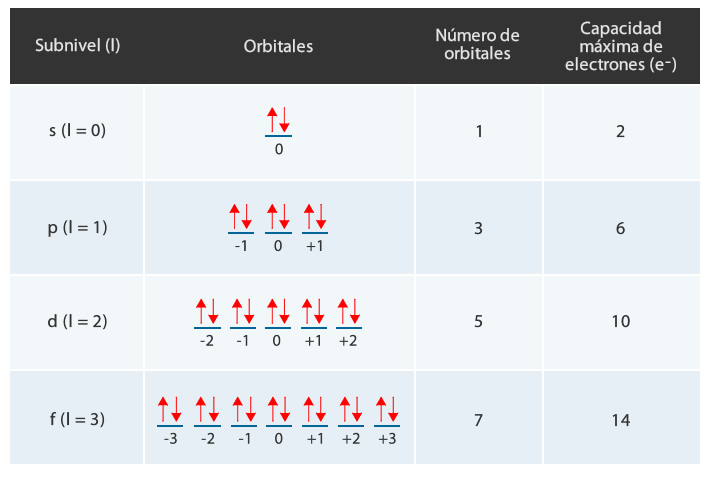
\includegraphics[width=1\textwidth]{numeros_cuanticos_5.jpg}
\caption{}
\end{figure}

\begin{figure}[h]
\centering
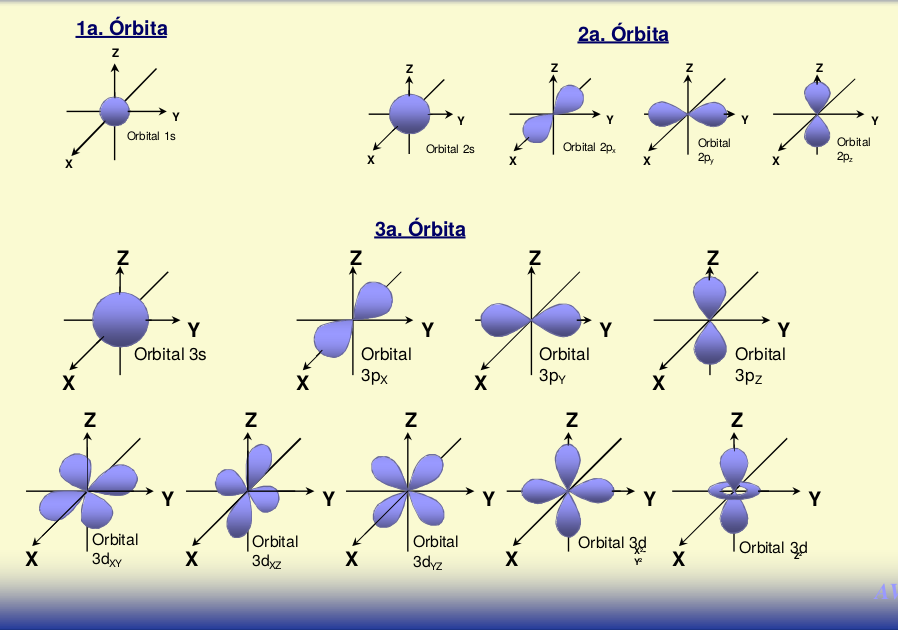
\includegraphics[width=1\textwidth]{orbitales.png}
\caption{}
\end{figure}

Durante la formación de un enlace, los orbitales atómicos se acercan y comienzan a solaparse, liberando energía a medida que el electrón de cada átomo es atraído por la carga positiva del núcleo del otro átomo. Entonces:

\begin{itemize}
    \item Cuanto mayor sea el solapamiento, mayor será el desprendimiento de energía y, por lo tanto, menor será la energía del orbital molecular. 
    
    \item Si el proceso de aproximación de los átomos continúa, los núcleos atómicos pueden llegar a repelerse mutuamente, lo que hace que la energía del sistema aumente.
    
    \item Esto significa que la máxima estabilidad (mínima energía) se alcanza cuando los núcleos se encuentran a una distancia determinada que se conoce como longitud de enlace.
\end{itemize}{}

En los sólidos, el enlace covalente es comúnmente encontrado en elementos con capas externas aproximadamente medio llenas. Un ejemplo notable es el carbono que forma solidos como el diamante, el grafeno y el grafito hasta complejas moléculas como los nanotubos de carbono. Los enlaces covalentes en el diamante son construidos desde una combinación lineal de orbitales 2s y tres orbitales 2p. Esto resulta en cuatro orbitales sp3 que se extienden en una configuración tetraédrica de los átomos de carbono.

La unión que constituye el Hidrógeno molecular es un ejemplo simple de un enlace covalente. La unión más intensa se presenta cuando los espines de ambos electrones son antiparalelos. La unión depende de la orientación relativa de los espines, no porque existan fuerzas dipolares magnéticas intensas entre ellos, sino porque el principio de exclusión de Pauli modifica la distribución de carga de acuerdo con la orientación de espines. La energía de Coulomb dependiente del espín se denomina interacción de intercambio.

\begin{figure}[h]
    \centering
    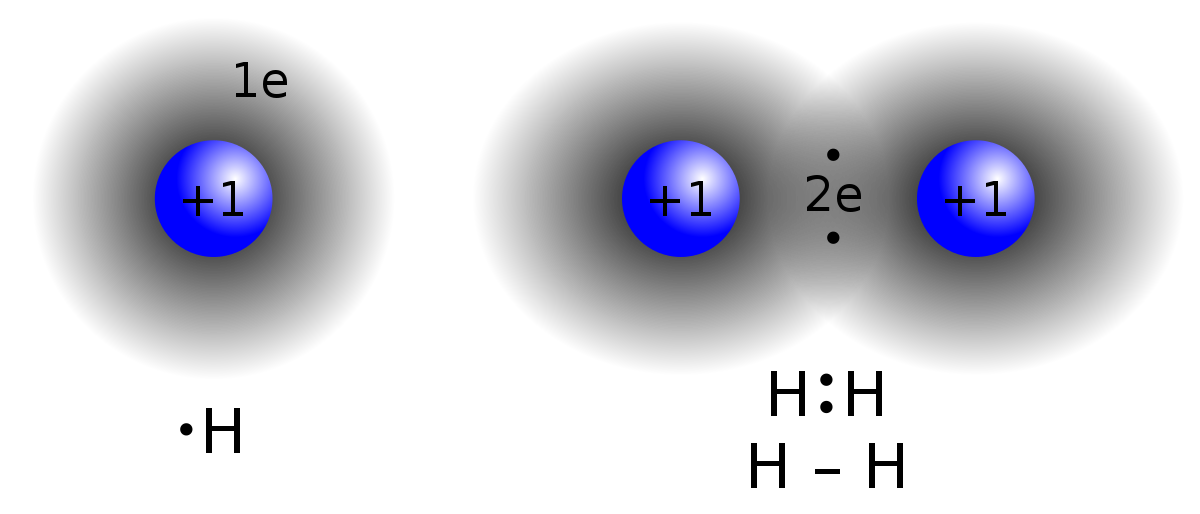
\includegraphics[width=0.8\textwidth]{hidrogeno_molecular.png}
    \label{Figura 1}
\end{figure}

Para entender mejor esto consideremos dos átomos de hidrógeno con sus núcleos a $R_{A}$ y $R_{B}$ y llamemos a $\abs{R_{A}- R_{B}} = R$. Conocemos, por supuesto, la solución de la ecuación de Schrodinger para cada uno de los átomos. Sea las funciones de onda del estado base $\phi_{A}$ y $\phi_{B}$ respectivamente. El operador hamiltoniano para la molécula de hidrógeno puede ser escrita entonces como:

\begin{equation}
    H= -\frac{\hbar^{2} \nabla^{2}_{1}}{2m_{e}}-\frac{\hbar^{2} \nabla^{2}_{2}}{2m_{e}}+\frac{e^{2}}{4\pi \epsilon_{0}}\left\lbrace{\frac{1}{R} + \frac{1}{\abs{r_{1}-r_{2}}} - \frac{1}{\abs{R_{A}-r_{1}}} - \frac{1}{\abs{R_{B}-r_{2}}} - \frac{1}{\abs{R_{A}-r_{2}}} - \frac{1}{\abs{R_{B}-r_{1}}} }\right\rbrace,
\end{equation}

donde $r_{1}$ y $r_{2}$ son las coordenadas de los electrones pertenecientes a los núcleos A y B respectivamente. Los primeros dos términos se refieren a la energía cinética de los dos electrones. Los operadores $\nabla^{2}_{1}$ y $\nabla^{2}_{2}$ actúan sólo en las coordenadas $r_{1}$ y $r_{2}$ respectivamente. Los términos electrostáticos contienen la repulsión entre dos núcleos y la repulsión entre los dos electrones, tanto como la atracción entre cada electrón y cada núcleo.

La solución a este problema no es simple. Podría simplificarse removiendo la interacción electrostática entre los dos electrones y así entonces el Hamiltoniano puede ser escrito como la suma de dos partes, una para cada electrón. Si los últimos dos términos en la ecuación 8 son removidos también, el problema puede ser resuelto por un producto de dos funciones de onda que son soluciones a dos Hamiltonianos atómicos individuales. La función de dos partículas puede escribirse de la forma $\phi(r_{1}, r_{2}) = \phi_{A}\phi_{B}$. \cite{Hofmann}

En realidad, esto no es muy cierto porque la función de onda no está en concordancia con el principio de exclusión de Pauli. Dado que los electrones son fermiones, la función de onda total debe ser antisimétrica respecto al intercambio de partículas y el producto de funciones de onda no cumple con este requerimiento. La función de onda total consiste en una parte espacial y una parte de espín y , por lo tanto, hay dos posibilidades para formar una función de onda antisimétrica. Podemos escoger una parte espacial simétrica y una parte espinorial antisimétrica o vice versa. Esto permite construir una función de onda espacial de la forma:

\begin{equation}
    \Phi_{\updownarrows}(r_{1}, r_{2})\ni \phi_{A}(r_{1})\phi_{B}(r_{2}) + \phi_{A}(r_{2})\phi_{B}(r_{1})
\end{equation}

\begin{equation}
    \Phi_{\upuparrows}(r_{1}, r_{2})\ni \phi_{A}(r_{1})\phi_{B}(r_{2}) - \phi_{A}(r_{2})\phi_{B}(r_{1})
\end{equation}

El signo positivo en la ecuación 9 nos da una función de onda espacial simétrica que podemos combinar con la parte espinorial antisimétrica igual a cero (el estado singlete); el signo negativo en la ecuación 10 resulta en una función de onda espacial antisimétrica para un espín simétrico con el espín igual a 1 (llamado el estado triplete).

La función de onda antisimétrica desaparece si $r_{1} = r_{2}$, esto significa que los electrones no pueden estar en el mismo lugar de forma simultánea. Esto conduce a una disminución de la densidad electrónica entre el núcleo y por tanto, a un estado antienlazante. Para el caso simétrico, del otro lado, los electrones tienen espines opuestos y pueden estar en el mismo lugar, lo cual permite una acumulación de carga entre el núcleo y por tanto, un estado de enlace. Ver figura 7.

\begin{figure}[h]
    \centering
    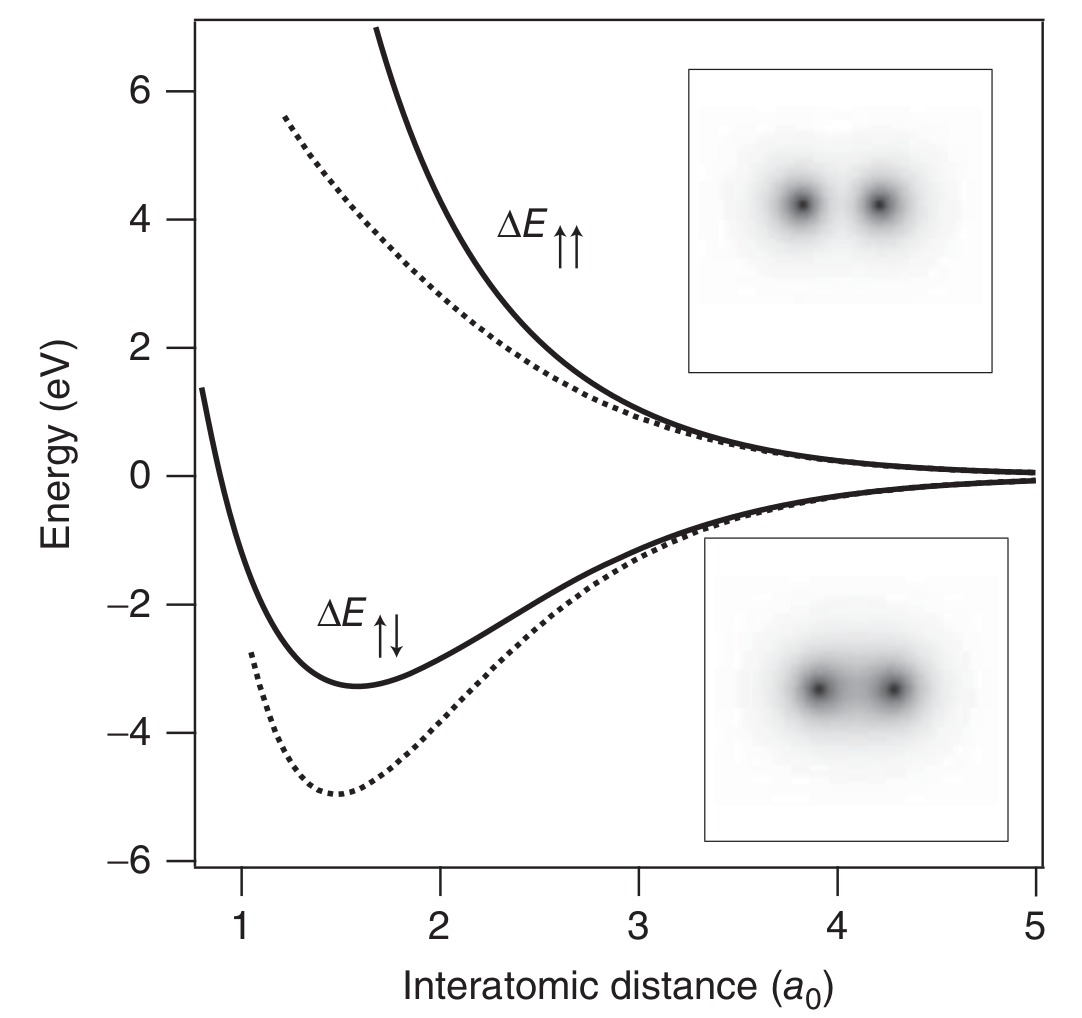
\includegraphics[width=0.8\textwidth]{Enlace_Covalente_2.png}
    \caption{Coordenadas de los osciladores}
    \label{Figura 1}
\end{figure}


Una forma aproximada de calcular los valores propios del Hamiltoniano en 8 fue sugerido por Heitler y London en 1927. La idea es usar las funciones de onda de la partícula individual 1s para un hidrógeno atómico para $\phi_{A}$ y $\phi_{B}$ desde una función de onda de dos electrones $\Phi(r_{1}, r_{2})$, el cual está dada por 9 y 10. Esas funciones de ondas podría no ser completamente correctas porque las funciones de onda atómicas pueden ser modificada por la presencia de otro átomo. Sin embargo, incluso si son aproximadamente correctas, podemos obtener los niveles de energía molecular como:

\begin{equation}
    E = \frac{\int \Phi^{*}(r_{1}, r_{2}) H \Phi(r_{1}, r_{2}) dr_{1}dr_{2}}{\int \Phi^{*}(r_{1}, r_{2})\Phi(r_{1}, r_{2}) dr_{1}dr_{2}}
\end{equation}{}

De acuerdo con el principio variacional en la mecánica cuántica, la energía resultante será más grande que la energía del estado base pero esta podrá ser una buena aproximación.

El cálculo es bastante largo  y no será mostrado aquí. Las energías resultantes para el estado base para el estado singlete y triplete pueden ser escritas como:

\begin{equation}
    E_{singlete} = 2E_{0} + \delta E_{\updownarrows}
\end{equation}

\begin{equation}
    E_{triplete} = 2E_{0} + \delta E_{\upuparrows}
\end{equation}

$E_{0}$ es el estado base de energía para el átomo de hidrógeno que aparece dos veces porque estamos considerando dos átomos. Las energías $\delta E_{\upuparrows}$ y $\delta E_{\updownarrows}$ son también mostradas en la figura. $\delta E_{\updownarrows}$ es siempre mayor que cero y no permite ningún enlace químico. $\delta E_{\upuparrows}$, por otro lado, muestra un mínimo por debajo de cero a aproximadamente 1.5 veces el radio de Bohr $a_{0}$. Este es el estado de enlace.

Para grandes distancias entre el núcleo, 12 y 13 pueden ser reescritas para obtener,

\begin{equation}
    E_{singlete} = 2E_{0} + C \pm X,
\end{equation}

Donde el signo + (-) es aplicado para el estado singlete (triplete). Ahora, el cambio en la energía sobre el enlace tiene dos partes, una que depende de las orientaciones relativas de los espines de los electrones, y una que no. La diferencia de energía entre los dos estados está dado por $2X$, donde $X$ es llamada energía de intercambio. En el caso de la molécula de hidrógeno, el intercambio en la energía es siempre negativo. La ecuación 14 es un extraordinario resultado porque significa que la energía del sistema depende de la orientación relativa de los espines, aunque esos espines no entren realmente en la ecuación de Schrodinger.

Nosotros encontraremos conceptos similares en el análisis del magnetismo donde el principio subyacente del ordenamiento magnético es muy similar el que vemos acá: La energía total del sistema de electrones depende de sus direcciones relativas de los espines a través de el intercambio de energía y, por lo tanto una ordenación particular de espín es predominante. Para dos electrones, el carácter "magnético" solamente dado por el signo de $X$. Para un $X$ negativo, el acople de dos espines opuestos es posible, resultando el caso antiferromagnético, mientras que un $X$ positivo puede permitir una situación en la que dos espines paralelos tengan la energía más baja, este sería el caso ferromagnético.

Observemos algunos tipos de enlaces covalentes: 

\begin{figure}[h]
    \centering
    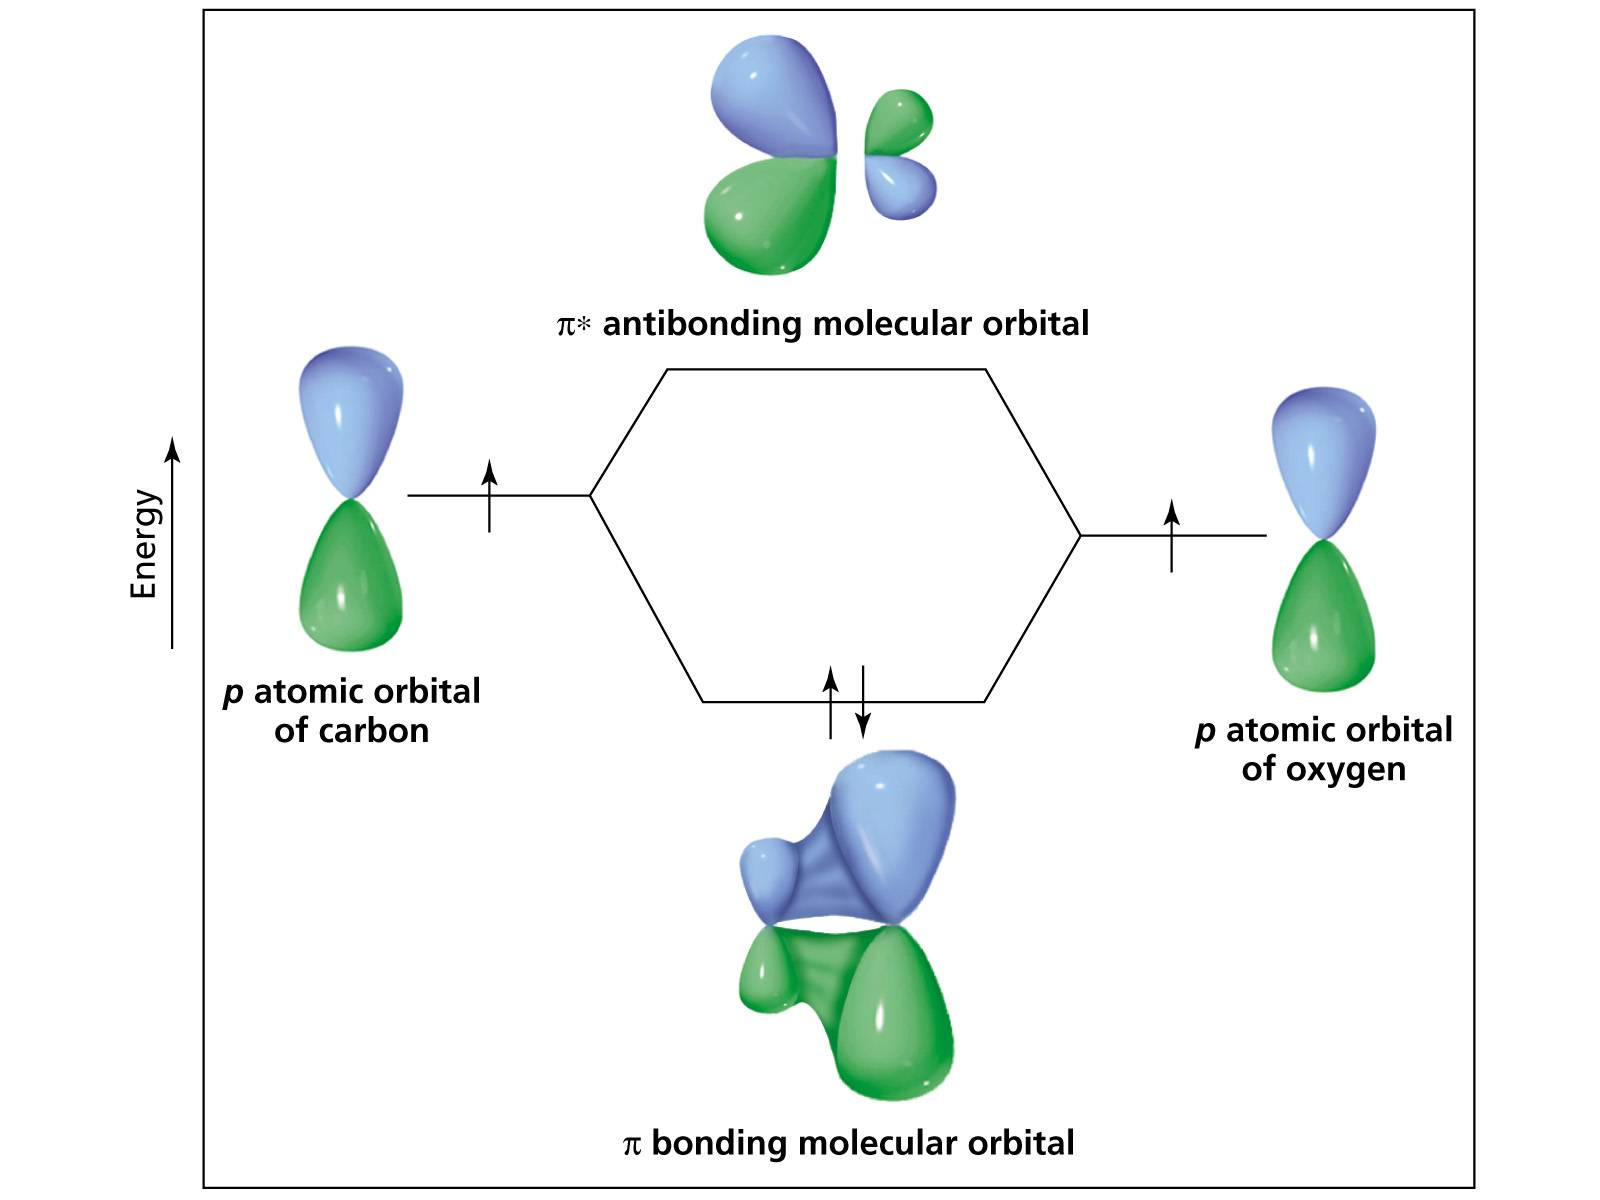
\includegraphics[width=0.7\textwidth]{pi.JPG}
    
    \label{Figura 1}
\end{figure}

De acuerdo a la forma como se encuentran las distribuciones de los orbitales a la hora de formar enlaces, se pueden establecer enlaces tipo sigma o tipo pi.

\begin{figure}[h]
    \centering
    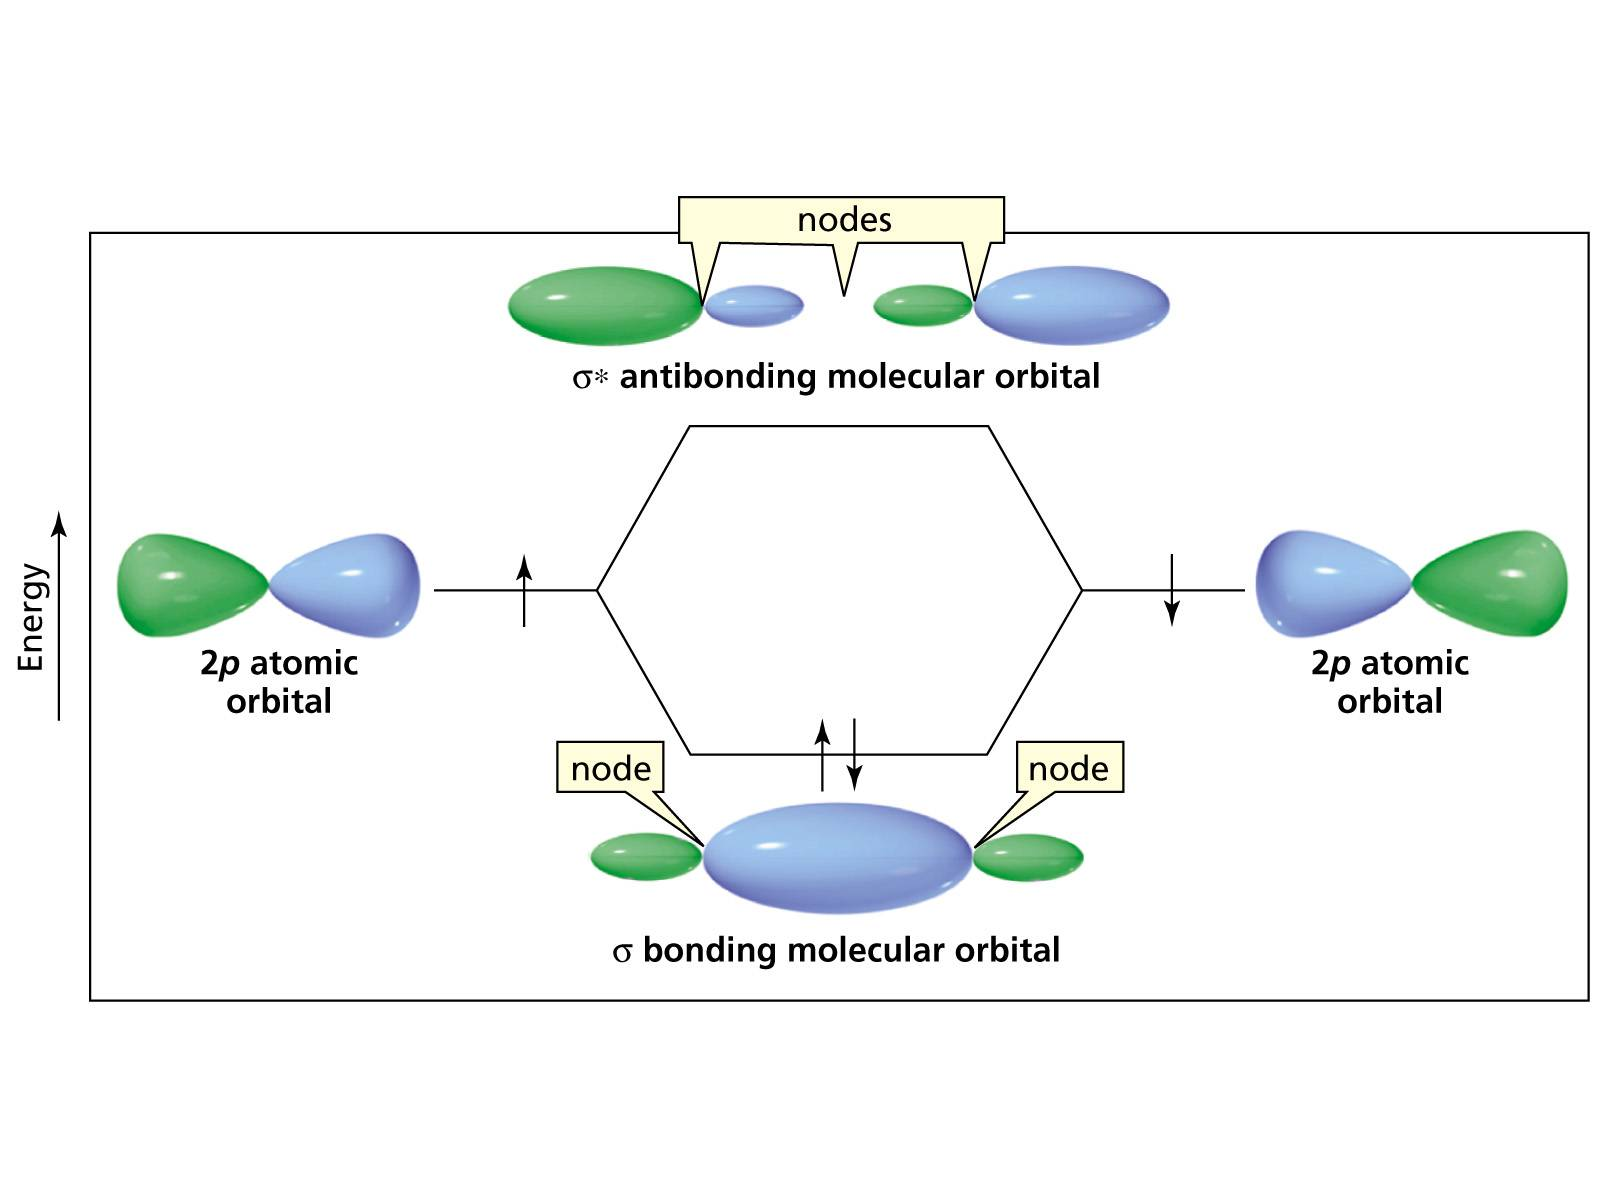
\includegraphics[width=1\textwidth]{sigma.JPG}
    
    \label{Figura 1}
\end{figure}

Para el caso del hidrógeno molecular o del floruro de hidrógeno:

\begin{figure}[h]
    \centering
    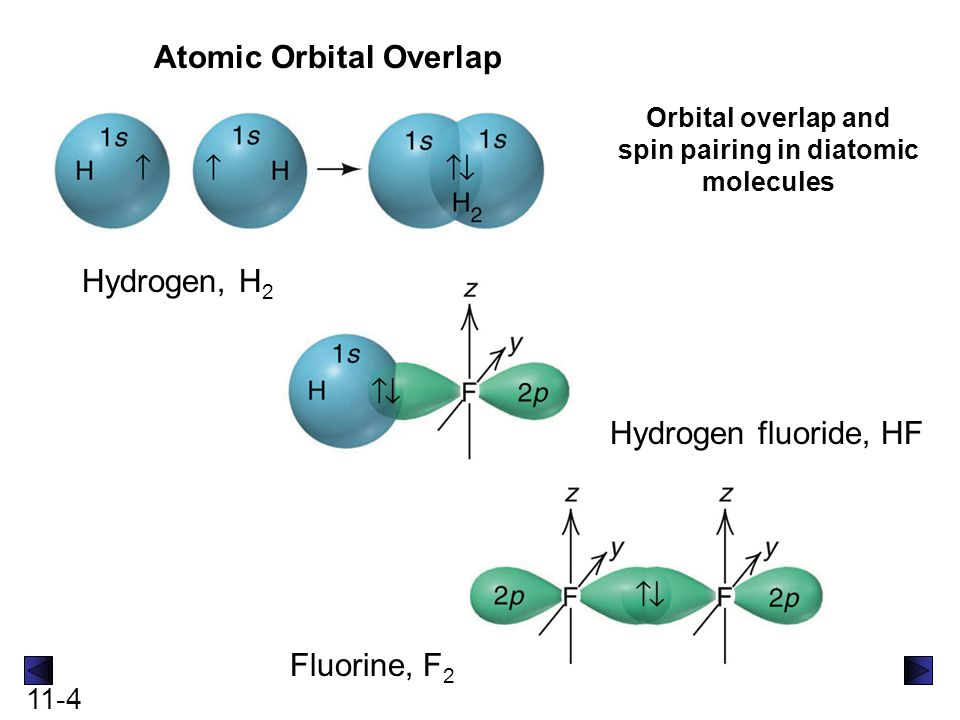
\includegraphics[width=0.8\textwidth]{hidrogeno_fluor.jpg}
    
    \label{Figura 1}
\end{figure}

\subsection{Sustancias con enlaces covalentes}

Las sustancias con enlaces covalentes forman en general dos clases de compuestos: \textbf{los cristales covalentes y sustancias moleculares}. 

Los cristales covalentes o atómicos, están constituidos por redes de enlaces covalentes que se extienden sin solución de continuidad en las tres direcciones del espacio terminando donde termina el cristal.

Las sustancias moleculares están formadas por moléculas discretas de mayor o menor tamaño, unidas entre sí por fuerzas intermoleculares.

Existen también sustancias covalentes con estructuras especiales que no se pueden encuadrar en ninguno de lo tipos establecidos.

\textit{Cristales covalentes} 

Estos cuerpos tienen todos sus átomos unidos entre sí mediante una red de enlaces covalentes que termina en los límites de la superficie del cristal. Son conocidos también con el nombre de cristales atómicos y sustancias reticulares.

Como ejemplo paradigmático de este tipo de sólidos tenemos el diamante, una forma alotrópica de carbono, Sus átomos están dispuestos en una red de tetraedros, con cada carbono rodeado por otros cuatro situados en los vértices de un tetraedro, y unidos a ellos por otros tantos enlaces covalentes.

El dióxido de silicio o sílice, $SiO_2$ es otro ejemplo de cristal covalente, en el que cada átomo de silicio está rodeado por cuatro átomos de oxígeno, cada uno de los cuales está unido a dos de silicio y así sucesivamente. Hay por tanto. Dos átomos de oxígeno por cada uno de oxígeno, y ello da razón de la fórmula, que es una formula empírica, no molecular. 


\newpage
\newpage

\section{Metales}

Los metales están caracterizados por una conductividad eléctrica elevada, y un gran número de electrones del metal se encuentran libres para moverse a través de él, normalmente, uno o dos por átomo. Los electrones disponibles para moverse se denominan electrones de conducción. Los electrones de valencia del átomo resultan ser los electrones de conducción en el metal. \cite{Kittel}

En algunos metales, la interacción de los iones con los electrones de conducción constituyen siempre una contribución considerable de la energía de enlace, pero la característica del enlace metálico es la disminución de la energía de los electrones de valencia del metal cuando se comparan con los átomos libres. 

\begin{figure}[h]
    \centering
    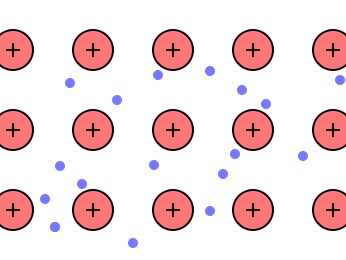
\includegraphics[width=0.8\textwidth]{metallicbonding.png}
    
    \label{Figura 1}
\end{figure}

En los metales, los electrones de valencia son removidos de los núcleos de los iones, pero en contraste con los solidos iónicos, no hay iones electronegativos para enlazarlos. Por lo tanto, son libres de moverse entre los núcleos. Esos no-localizados electrones de valencia están involucrados con la conducción de la electricidad y son llamados electrones de conducción. Se puede esperar que los metales se formen de elementos para los cuales el costo de energía de remover los electrones más  externos no sea tan grande. Sin embargo, la remoción siempre cuesta algo de energía que debe ser mayor que la compensada por el enlace. Explicar la ganancia de la energía del enlace en una imagen intuitiva es difícil pero podemos hacerlo posible. El razonamiento deberá conducir a algún tipo de reducción en la energía.

Una contribución menor es la energía cinética de los electrones de conducción. Considere la contribución en la energía cinética del Hamiltoniano, $T = \frac{\hbar^{2} \nabla^{2}}{2m_{e}}$. Un elemento de la matriz $\braket{\Phi|T|\Phi}$ mide la energía cinética de la partícula $T\Phi$ es proporcional a la segunda derivada espacial de la función de onda, esto es, la curvatura. Para un electrón que está localizado en el átomo, la curvatura de la función de onda es mucho mayor para un electrón libre en las cercanías de los átomos del metal y de ahí de de donde viene la ganancia en la energía.

La otra contribución a la energía del electrón es la energía potencial. Se podría pensar que el potencial electrostático promedio para cualquier electrón libre en un sólido es casi cero Porque hay tantos otros electrones como iones con la misma cantidad de carga. Pero esto está mal. En efecto, los electrones sienten un potencial atractivo. La razón es otra vez culpa del principio de Pauli que, en resumidas cuentas, no permite dos electrones con la misma dirección de espín estar en el mismo lugar. Adicional a esto, hay una interacción directa de Coulomb entre los electrones que hace que ellos eviten a los otros. 

Podemos también entender por qué los metales prefieren estructuras de empaquetamiento compacto. Primero que todo, el enlace metálico no tiene una dirección preferencial. Segundo, las estructuras compactas aseguran mayor superposición posible entre los orbitales de valencia de los átomos, maximizando la no-localización de los electrones y de este modo la ganancia de energía cinética. Las estructuras también maximizan el numero de vecinos más cercanos para cada átomo dado, otra vez entregando unos estados fuertemente no-localizados.

Típicamente, el enlace metálico no es tan fuerte como el covalente o el iónico pero este acumula una cantidad de voltaje por átomo.

\begin{figure}[h]
    \centering
    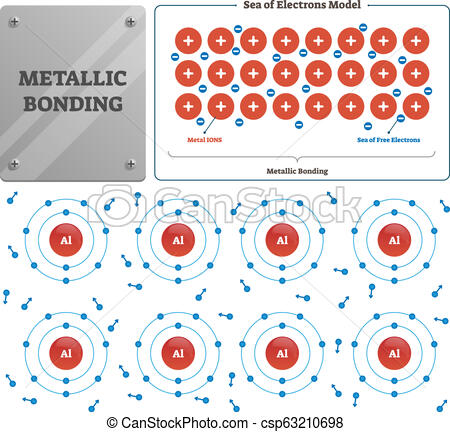
\includegraphics[width=0.8\textwidth]{metallic-bonding-vector-illustration-drawing_csp63210698.jpg}
    
    \label{Figura 1}
\end{figure}

\textbf{En resumen},

La combinación de dos fenómenos da lugar a un enlace metálico: la deslocalización de los electrones y la disponibilidad de un número mucho mayor de estados de energía deslocalizados que de electrones deslocalizados. [Esta clarificación es necesaria] Esta última podría llamarse deficiencia de electrones.

En 2D:  El grafeno es un ejemplo de unión metálica bidimensional. Sus enlaces metálicos son similares a los enlaces aromáticos en benceno, naftaleno, antraceno, ovaleno, etc.

En 3D: La aromaticidad del metal en grupos de metal es otro ejemplo de deslocalización, esta vez a menudo en entidades tridimensionales. Los metales llevan el principio de deslocalización al extremo y se podría decir que un cristal de un metal representa una molécula única sobre la cual todos los electrones de conducción están deslocalizados en las tres dimensiones. Esto significa que dentro del metal uno generalmente no puede distinguir las moléculas, por lo que la unión metálica no es ni intra ni intermolecular. "Nonmolecular" quizás sería un término mejor. La unión metálica es en su mayoría no polar, porque incluso en las aleaciones hay poca diferencia entre las electronegatividades de los átomos que participan en la interacción de la unión (y, en metales elementales puros, ninguna). Por lo tanto, el enlace metálico es una forma comunal extremadamente deslocalizada de enlace covalente. En cierto sentido, la unión metálica no es un tipo "nuevo" de unión, por lo tanto, y describe la unión solo como presente en un trozo de materia condensada, ya sea cristalina, líquida o incluso vidrio. Los vapores metálicos, por el contrario, suelen ser atómicos (Hg) o, a veces, contienen moléculas como Na2, unidas por un enlace covalente más convencional. Es por esto que no es correcto hablar de un solo 'enlace metálico'.

La deslocalización es más pronunciada para los electrones s y p. Para el cesio es tan fuerte que los electrones están virtualmente libres de los átomos de cesio para formar un gas restringido solo por la superficie del metal. Para el cesio, por lo tanto, la imagen de los iones Cs + mantenidos juntos por un gas electrónico cargado negativamente no es demasiado inexacta. [5] Para otros elementos, los electrones son menos libres, ya que aún experimentan el potencial de los átomos metálicos, a veces con bastante fuerza. Requieren un tratamiento mecánico cuántico más intrincado (por ejemplo, una fuerte unión) en el que los átomos se consideran neutros, al igual que los átomos de carbono en el benceno. Para d- y especialmente para los f-electrones, la deslocalización no es fuerte en absoluto y esto explica por qué estos electrones pueden seguir comportándose como electrones no pareados que retienen su espín, lo que agrega propiedades magnéticas interesantes a estos metales.


\section{Enlace de Hidrógeno}

La fuerza por puente de hidrógeno o enlace de hidrógeno \textbf{es la fuerza eminentemente electrostática atractiva entre un átomo electronegativo y un átomo de hidrógeno unido covalentemente a otro átomo electronegativo.} Resulta de la formación de una fuerza carga-dipolo con un átomo de hidrógeno unido a un átomo de nitrógeno, oxígeno o flúor (de ahí el nombre de "enlace de hidrógeno", que no debe confundirse con un enlace covalente a átomos de hidrógeno. \cite{Kittel}


\begin{figure}[h]
    \centering
    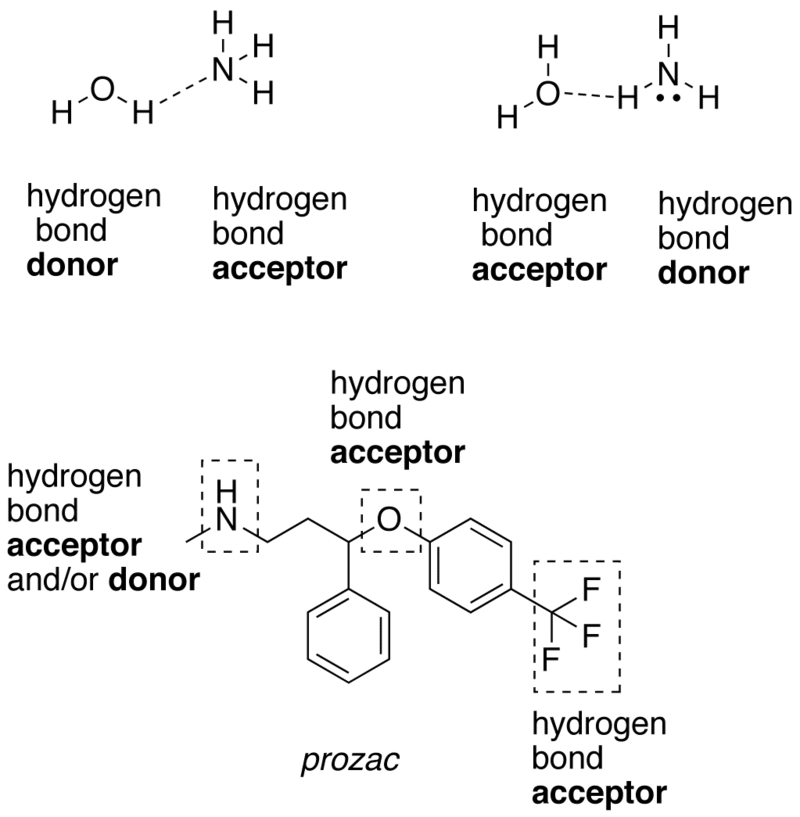
\includegraphics[width=0.8\textwidth]{Enlace_de_Hidrogeno_2.png}
    
    \label{Figura 1}
\end{figure}

La energía de un enlace de hidrógeno (típicamente de 5 a 30 kJ/mol) es significativamente menor a la de los enlaces covalentes débiles (155 kJ/mol), y un enlace covalente típico es sólo 20 veces más fuerte que un enlace de hidrógeno intermolecular. Estos enlaces pueden ocurrir entre moléculas (intermolecularidad), o entre diferentes partes de una misma molécula (intramolecularidad). 

El enlace de hidrógeno es una fuerza electrostática dipolo-dipolo fija muy fuerte cuando están muchas moléculas unidas, ya que da gran estabilidad, pero más débil que el enlace covalente o el enlace iónico. La fuerza del enlace de hidrógeno se ubica en algún lugar intermedio entre un enlace covalente y una fuerza de Van der Waals (fuerza de dispersión). Este tipo de enlace ocurre tanto en moléculas inorgánicas tales como el agua, y en moléculas orgánicas como el ADN.

El enlace de hidrógeno intermolecular es responsable del punto de ebullición alto del agua (100°C). Esto es debido al fuerte enlace de hidrógeno, en contraste a los otros hidruros de calcógenos. El enlace de hidrógeno intramolecular es responsable parcialmente de la estructura secundaria estructura terciaria y estructura cuaternaria de las proteínas y ácidos nucleicos. 


\section{Radio Atómico}

Las distancias entre los átomos de los cristales pueden medirse con mucha exactitud mediante difracción de rayos X, con frecuencia hasta una parte en $10^5$. ¿Podremos decir que la distancia observada entre átomos puede asignarse parcialmente a un átomo A y a un átomo B? ¿Puede asignarse un significado definido  al radio de un átomo o de un ión, con independencia de la naturaleza o estructura del cristal?

Estrictamente, la respuesta es no. La distribución de cargas alrededor de un átomo no está limitada por un contorno específico rígido. No obstante, el concepto de radio atómico es fructífero para la predicción de espaciados o separaciones interatómicas. Además, la configuración electrónica de los átomos constituyentes con frecuencia pueden deducirse por comparación de los valore medidos y predichos de las constantes de red.

Para hacer predicciones de las constantes de la red, es conveniente asignar conjuntos de radios coherentes a diversos tipos de enlaces.

%\newpage

\section{Tablas periódicas con información de interés}


\begin{figure}[H]
    \centering
    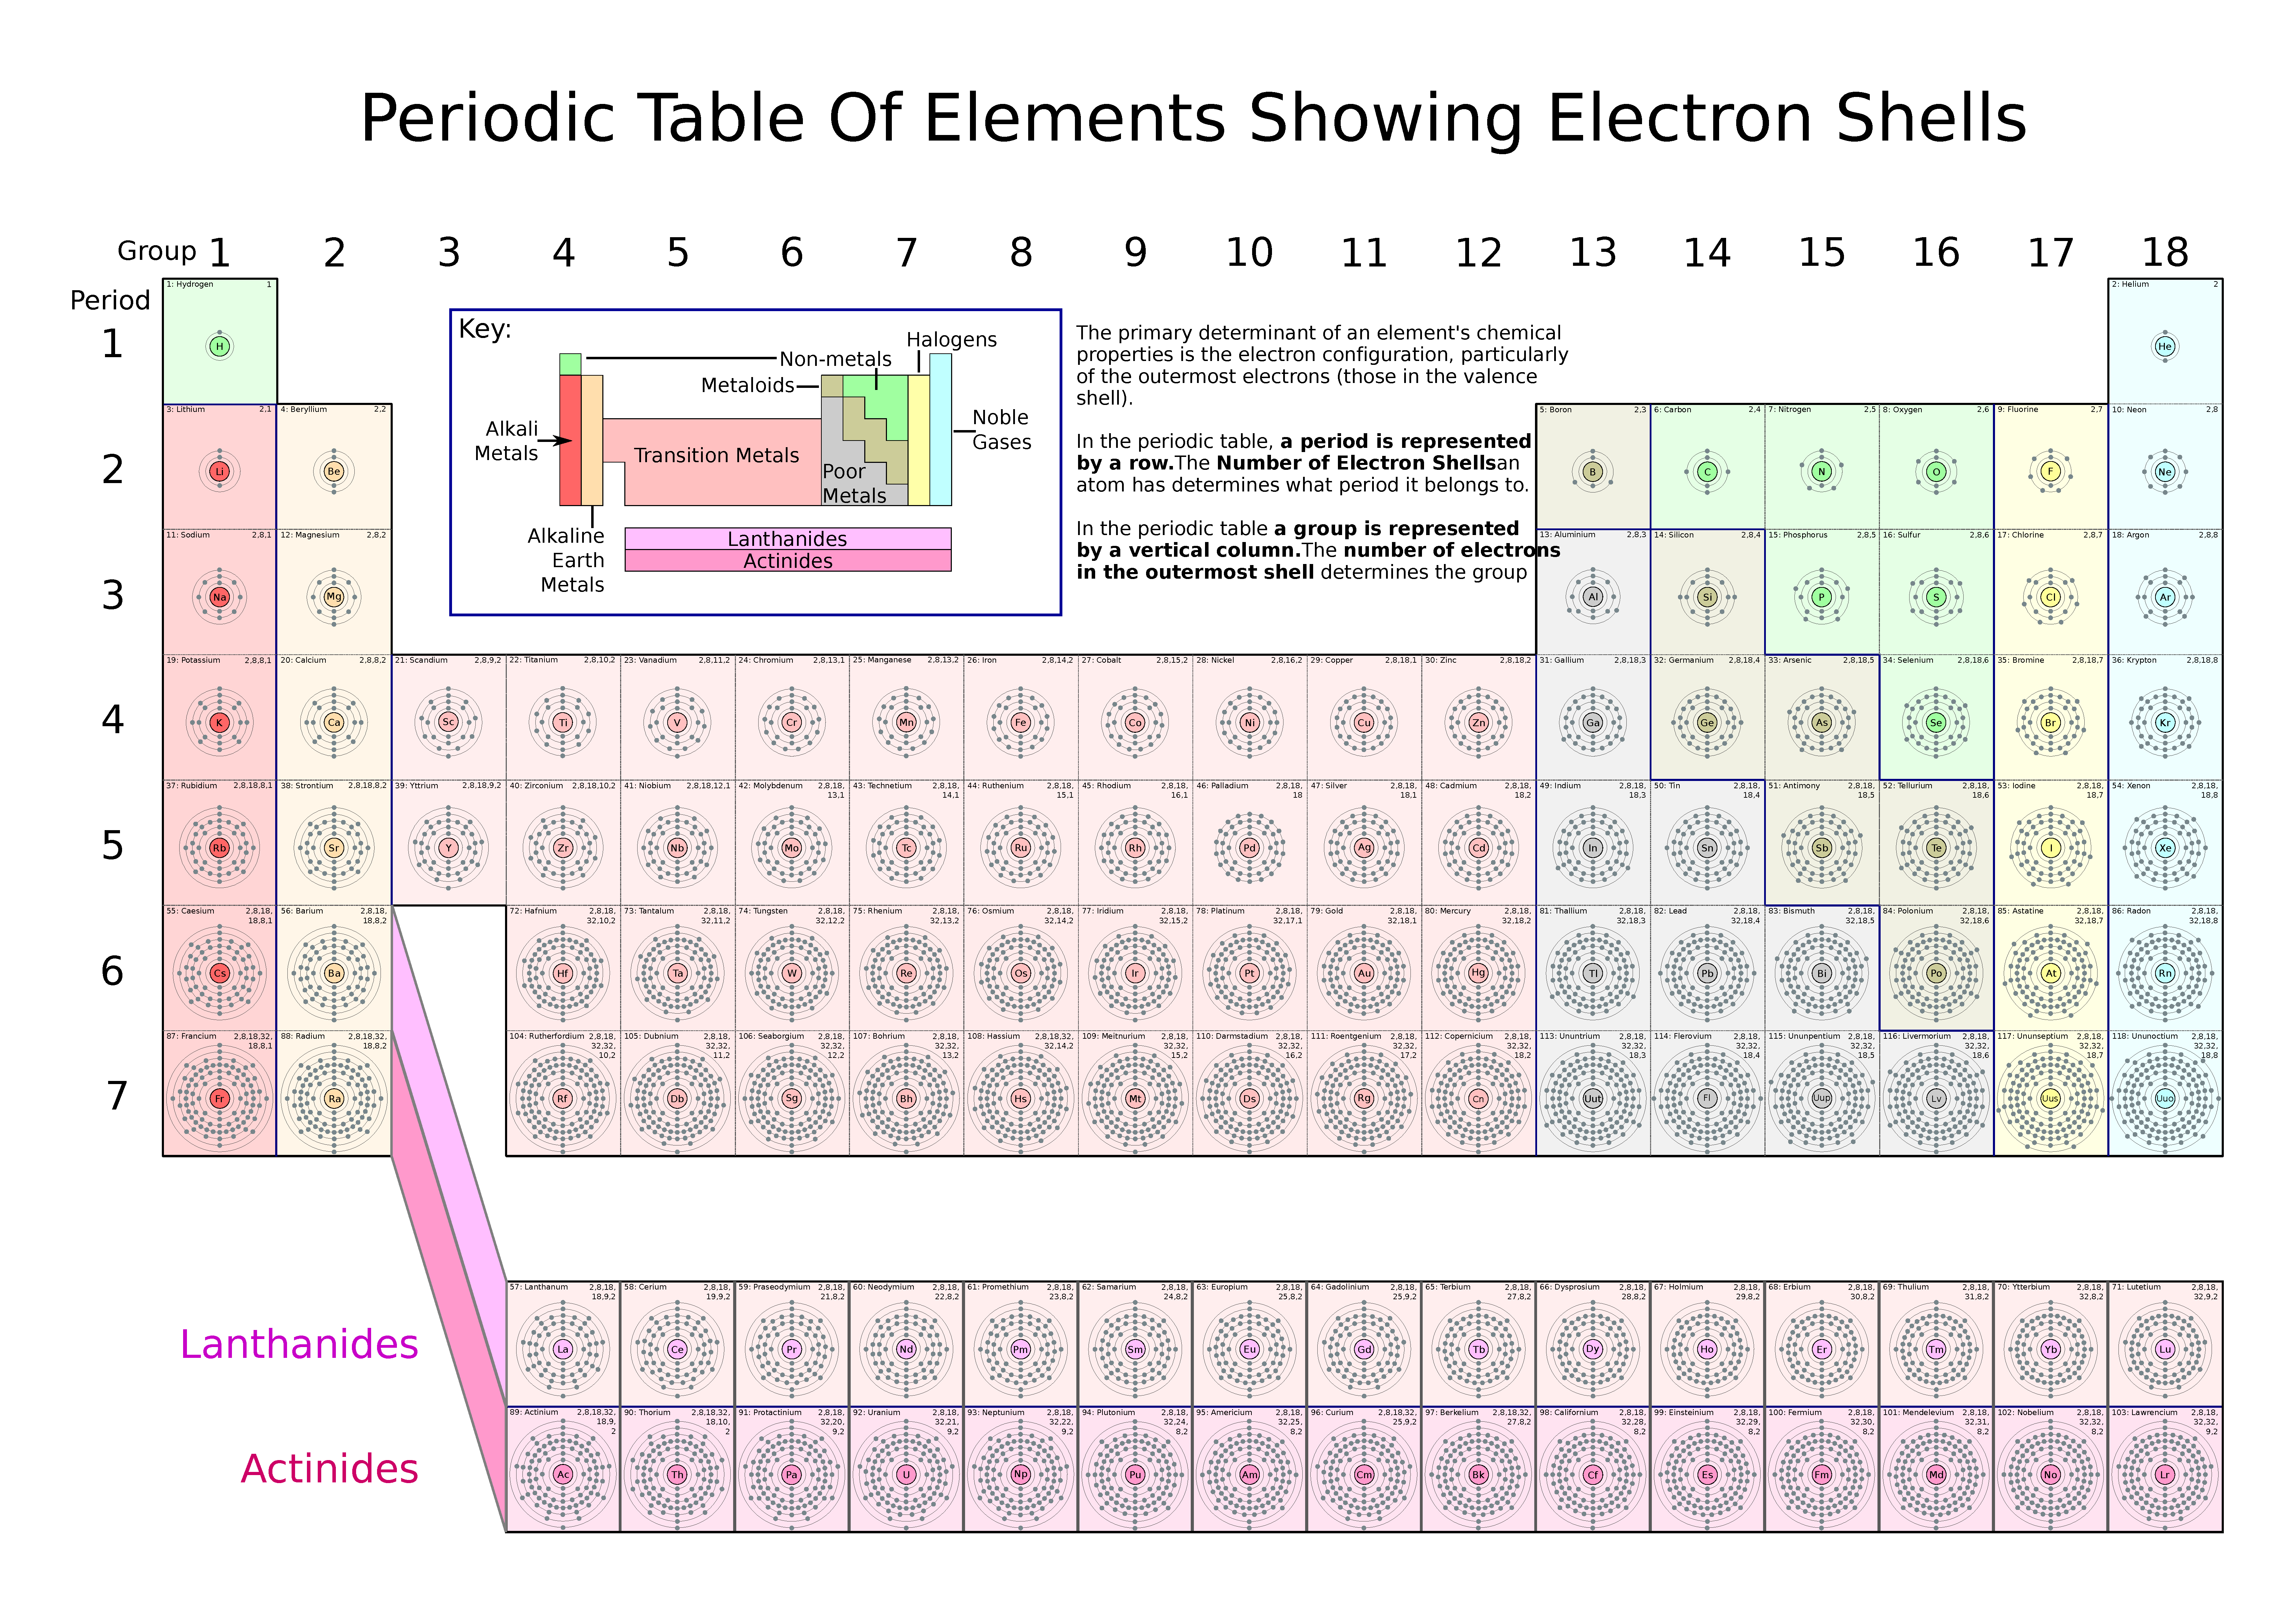
\includegraphics[width=1\textwidth]{Periodic_Table_of_Elements_showing_Electron_Shells_(2011_version).pdf}
 \end{figure}

\begin{figure}[H]
    \centering
    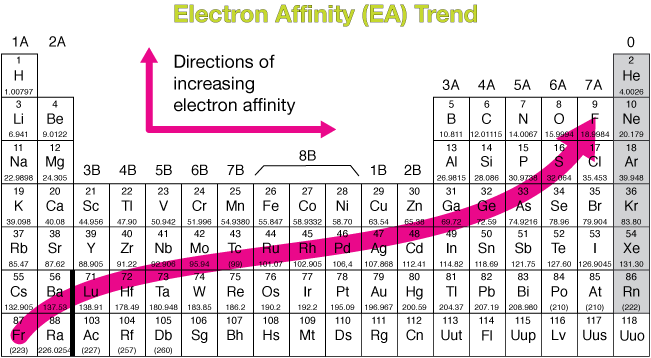
\includegraphics[width=1\textwidth]{ElectronAffinityTrend.png}
    \end{figure}

\begin{figure}[H]
    \centering
    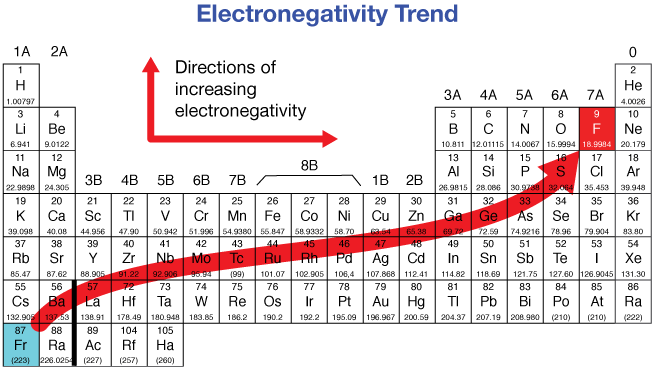
\includegraphics[width=1\textwidth]{qauzvgRRrWMhrcf1oYAA_ElectronegativityTrendFigure.png}
    \end{figure}


\begin{figure}[H]
    \centering
    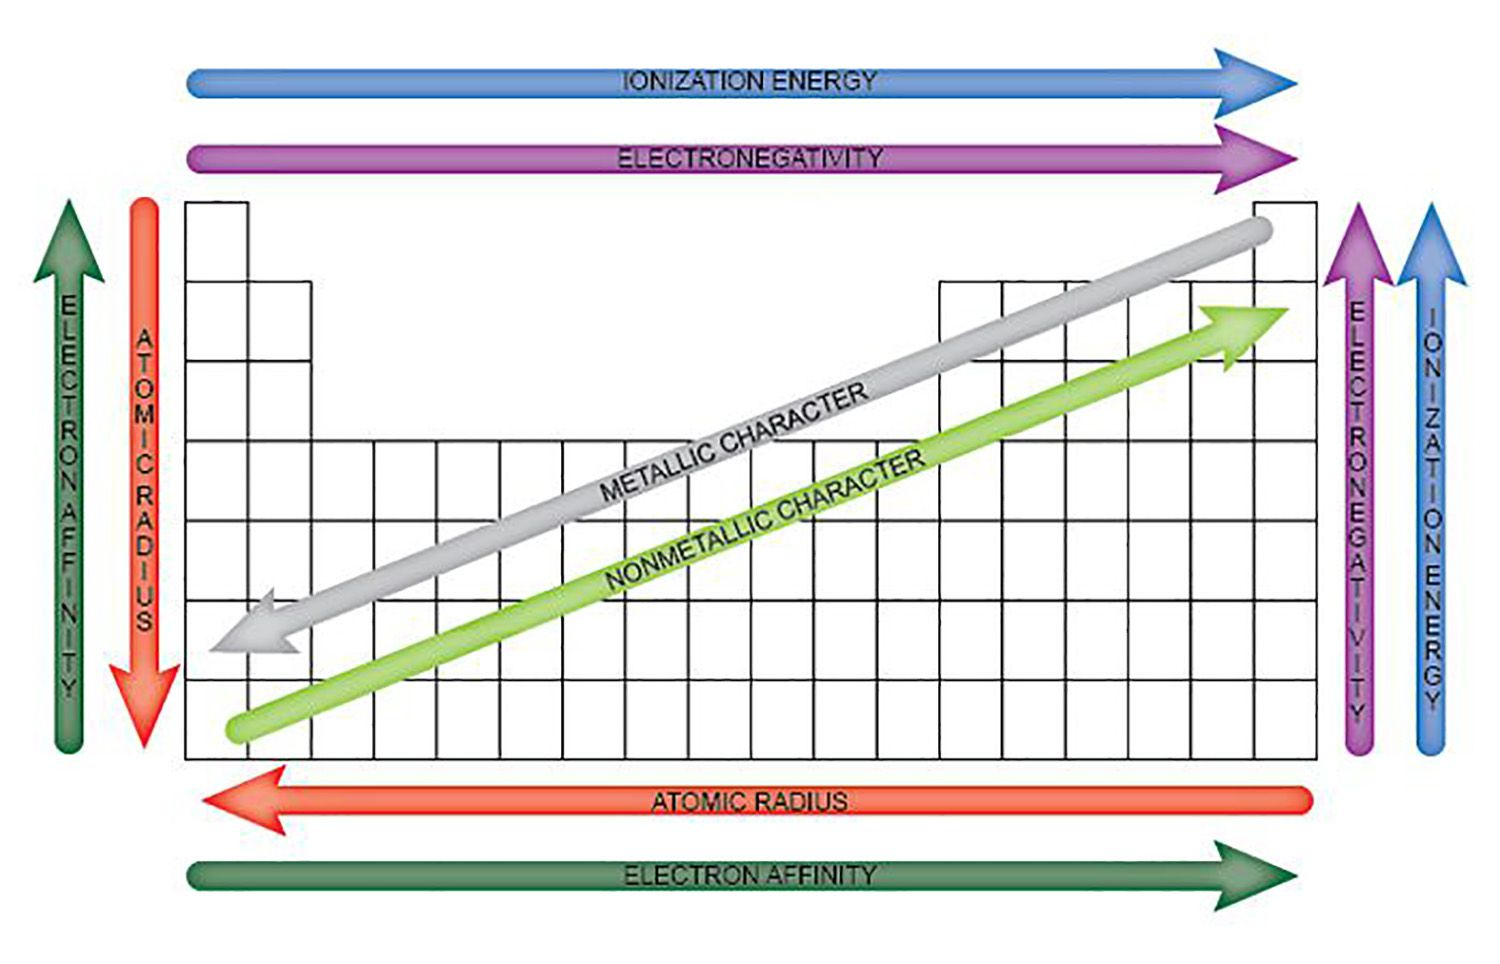
\includegraphics[width=1\textwidth]{ELECTRONEGAjfjksdgfjg.jpg}
    \end{figure}

   \newpage
   
   
\bibliographystyle{abbrv}
\bibliography{referencias}

\end{document}
